\subsection{Reprezentacja rozwiązania}
Rozwiązaniem problemu jest permutacja długości liczby ofert.
Za oferty przyjęte jako zaakceptowane wybieramy zgodnie z kolejność występowania w permutacji z pominięciem tych, których towary pokrywały się z towarami jakiejs oferty wcześniej występującej.

\subsection{Funkcja celu}
Zgodnie z reprezentacją sumujemy te ceny tych ofert, które zostały zaakceptowane. Przeglądamy permutacje od lewej do prawej i wybieramy te oferty, których towary nie zostały wykupione przez wcześniejsze oferty.

\subsection{Rozwiązanie}
Do rozwiązania tego problemu użyliśmy algorytmu algorytmu SGA.
Jego parametry najcześciej na 200 iteracji i populacje o rozmiarze 40.
Podczas każdej iteracji, nie wymienialiśmy całej populacje, a jedynie 10 osobników.

\subsubsection{Krzyżowanie}
Do krzyżowania użyliśmy lekko zmodyfikowanego algorytmu PMX.
Założyliśmy, że funkcja celu zależy bardziej od elementów o mniejszym indeksie w permutacji niż większym.
Elementy o mniejszy indeksie są bardziej preferowane co wynika z funkcji celu, a oferty o dalszych indeksach mogą być często wogle nie brane do rozwiazania.
Dlatego staramy się, aby wymieniamy przez operator PMX środkowy segment zaczynał się cześciej w niskich indeksach.


Wprowadzona modyfikacja polega na wyborze punktów $a$ i $b$ będących przedziałem wymienianego środkowego segmentu.
W pierwotnej wersji były losowane dwie liczby $x, y$ i na ich podstawie wyliczane punkty $a$, $b$.
\begin{equation}
    a = min(x, y) \cdot n \ \wedge \ b = max(x, y) \cdot n \ \ \hbox{gdzie n to długość permutacji}
\end{equation}
W zmodyfikowanej wersji punty były wyliczane w poniższy sposób.
\begin{equation}
    a = min(x, y)^2 \cdot n \ \wedge \ b = max(x, y) \cdot n
\end{equation}

\subsubsection{Mutacja}
Wybrana przez nas mutacja jest dość prosta, ale okazała się znacząco poprawiać wyniki.
Polega na cyklicznym przesunięciu całej permutacji o jeden element w lewo. 
W ten sposób oferta, która była pierwsz w permutacji staje się ostatnio. 
Z zasady działania funkcji celu wielmu, że pierwsza oferta jest zawsze wybierana, a ostatnio dość rzadko dzięki czemu ta mutacja dość znacząco zmieniała osobniki.

\subsubsection{Wymiana}
Wymiana elemntów polega na zastąpieniu najgorszych osobników stałą liczbą, ustawianą jako parametr, zmutowanych i skrzyżowancyh osobników.
Dzięku odpowiednim doborze tej liczby populacja zawsze pamiętała stare najlepsze osobniki przez pewną liczba iteracji co wpływało na poprawę znajdowanych wyników.

\subsubsection{Warunek stopu}
Na początku za warunek stopu przyjeliśmy unikalność wszystkich elementów.
Gdy wartości funkcji celu dla wszystkich elementół w populacji były takie same to przerywaliśmy algorytm.
Takie podejście okazało się jednak błędne, gdyż pomimo iż wartości funkcji celu były takie same osobniki były znacząco różne w sensie permutacji i pozwolenie im na dalsze iteracje poprawiło trochę wyniki.

\subsection{Wyniki}
Wyniki przestawione są na wykresach (\ref{wyk:sga1}, \ref{wyk:sga2}, \ref{wyk:sga3}, \ref{wyk:sga4}).
Na niebiesko zaznaczono wynik dla algorytmu SGA dla kolejnych iteracji.
Na zielono zaznaczono najlepszy wynik algorytmu losowego, który wybierał wynik z takiej samej puli losowych osobników ile lącznie przegląda SGA.


Na wykresach \ref{wyk:sga1}, \ref{wyk:sga2} i \ref{wyk:sga3} algortym kończył swoje działanie gdy wszsytkie osobniki w populacji były unikalne pod względem wartości funkcji celu.
Na wykresie \ref{wyk:sga4} przestawiona jest wersja algorytmu, która kończyła poszukiwania  po ustalonej liczbie iteracji.
Podczas algorytmu próbowaliśmy również podmieniać niektóre stare osobniki nowymi losowymi gdy wszystkie poprzednie były już unikalne.
Jak widać takie podejście okazało się być lepsze od poprzedniego gdyż algorytm po pewnym czasie działania znajdował troche lepsze rozwiązanie.


\begin{figure}[ht!]
    \centering
    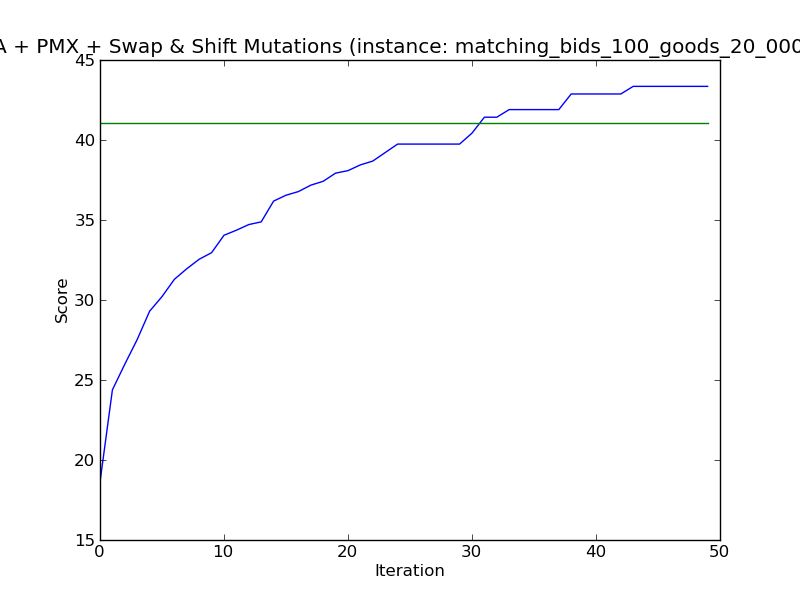
\includegraphics[width=10cm]{wykresy/matching_bids_100_goods_20_0000_txt_1.png}
    \caption{Wykres dla problemu 'matching' o parametrach 100 ofert i 20 towarów.}
    \label{wyk:sga1}
\end{figure}

\begin{figure}[ht!]
    \centering
    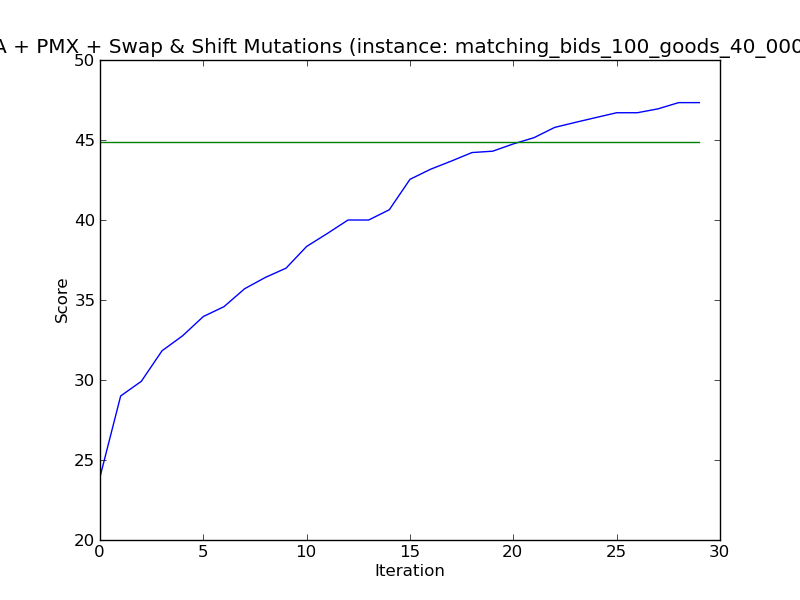
\includegraphics[width=10cm]{wykresy/matching_bids_100_goods_40_0000_txt_3.png}
    \caption{Wykres dla problemu 'matching' o parametrach 100 ofert i 40 towarów.}
    \label{wyk:sga2}
\end{figure}

\begin{figure}[ht!]
    \centering
    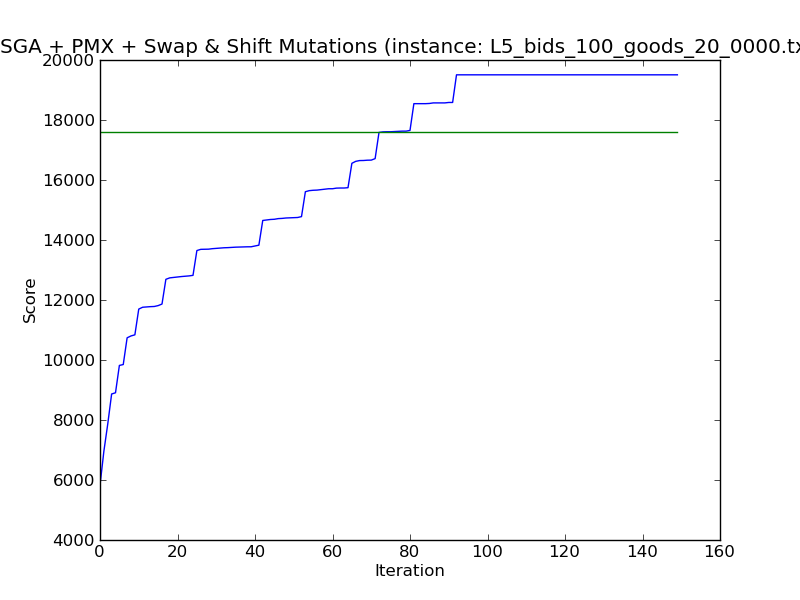
\includegraphics[width=10cm]{wykresy/L5_bids_100_goods_20_0000_txt_1.png}
    \caption{Wykres dla problemu 'L5' o parametrach 100 ofert i 20 towarów.}
    \label{wyk:sga3}
\end{figure}

\begin{figure}[ht!]
    \centering
    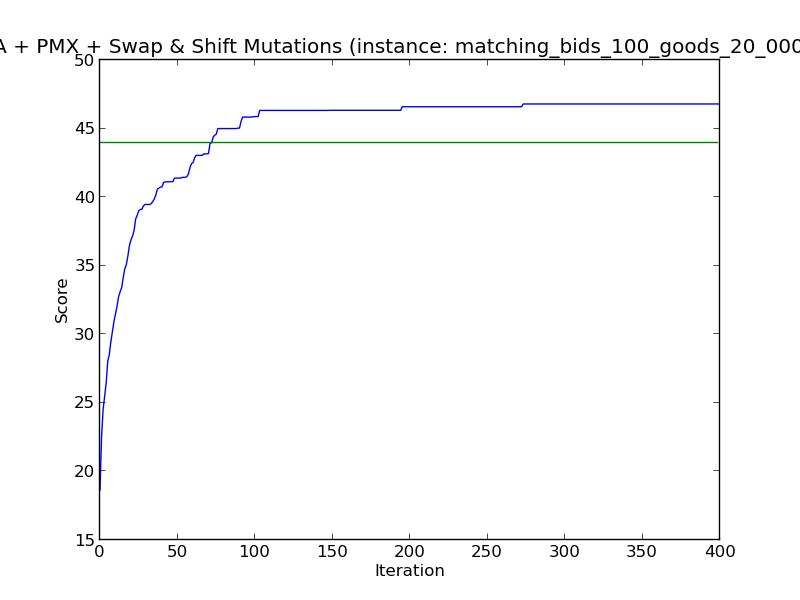
\includegraphics[width=10cm]{wykresy/matching_bids_100_goods_20_0000_txt_uniq.png}
    \caption{Wykres dla problemu 'matching' o parametrach 100 ofert i 20 towarów.}
    \label{wyk:sga4}
\end{figure}


